\documentclass[UTF8, 11pt, oneside]{ctexart}

\usepackage{float}

\usepackage{geometry}
\geometry{a4paper,left=2cm,right=2cm,top=2cm,bottom=1cm}

\usepackage{graphicx}

\usepackage{hyperref}
\hypersetup{colorlinks=true, linkcolor=red}

\linespread{1.6}


\def\articletitle{小仙女说得对,就不应该生娃}

\usepackage{fancyhdr}
\usepackage{ifthen}
\pagestyle{fancy}
\fancyhf{}
\setlength{\headheight}{14pt}
\fancyhead[R]{\ifthenelse{\value{page}>1}{\thepage}{}}
\fancyhead[C]{\ifthenelse{\value{page}>1}{\articletitle}{}}
\renewcommand\headrulewidth{0pt}

\usepackage{tcolorbox}
\tcbuselibrary{skins}


\newcommand{\zd}[1]{\textbf{\textcolor[RGB]{123,12,0}{#1}}} % 重点

\newcommand{\yh}[1]{% 引用
    \begin{tcolorbox}[enhanced,
        frame hidden, interior hidden,
        before skip = 5mm, left skip=10mm,
        borderline west={5pt}{0pt}{gray!50}]
        #1
    \end{tcolorbox}
}

\newcommand{\biaoti}[1]{% 标题
    \section*{#1}
}

\begin{document}

\begin{center}
    \LARGE{\articletitle\footnotemark}
\end{center}
\footnotetext{
    原文出自公众号“老端”的文章 《\href{https://mp.weixin.qq.com/s/1dODBxps2BxwAnZA3Ocqag}{\articletitle}》
}

前两天我发了一篇小文《女儿说,将来想生五个娃》,顺便谈了谈对于社会上充斥着大龄剩女的思考,结果评论区就炸锅了,文章点击量也不高,但后台评论多达上千条,你能看到的只是一小部分,因为很多言论已经被系统过滤掉了,还有些太激进的我没有放出来。

为什么这些小仙女会如此激动地反击我呢?因为我的文章在她看来,是在质疑她的信仰,这些“拳师”就像一神教的祭司,特别讲究信仰的不可置疑性,我的这些言论,在她看来就是当着犹太人的面说巴勒斯坦人好话,这是她们万万不能接受的。

她们有一套自己的话术来解释问题,比如为什么自己不婚不育?她们的话术是中国男人不行!要么太穷太屌丝,要么不顾家不管孩子,要么喜欢出轨约炮。总之,问题都在别人身上,自己是不可能给这些人生孩子的。

可是她们能看上的那些男人,早就娶妻生子了,就算单身也看不上她啊。按照正常思路,卖不掉的菜可以打折处理掉,可她是不可能降低标准的,本着宁缺毋滥的精神,一直坚持高价不动摇。网友戏称:她们的这些奇葩需求,能够满足的估计就只剩下“杀猪盘”了。

下面这幅漫画非常精准地描绘了这些人:

\begin{figure}[H]
    \centering
    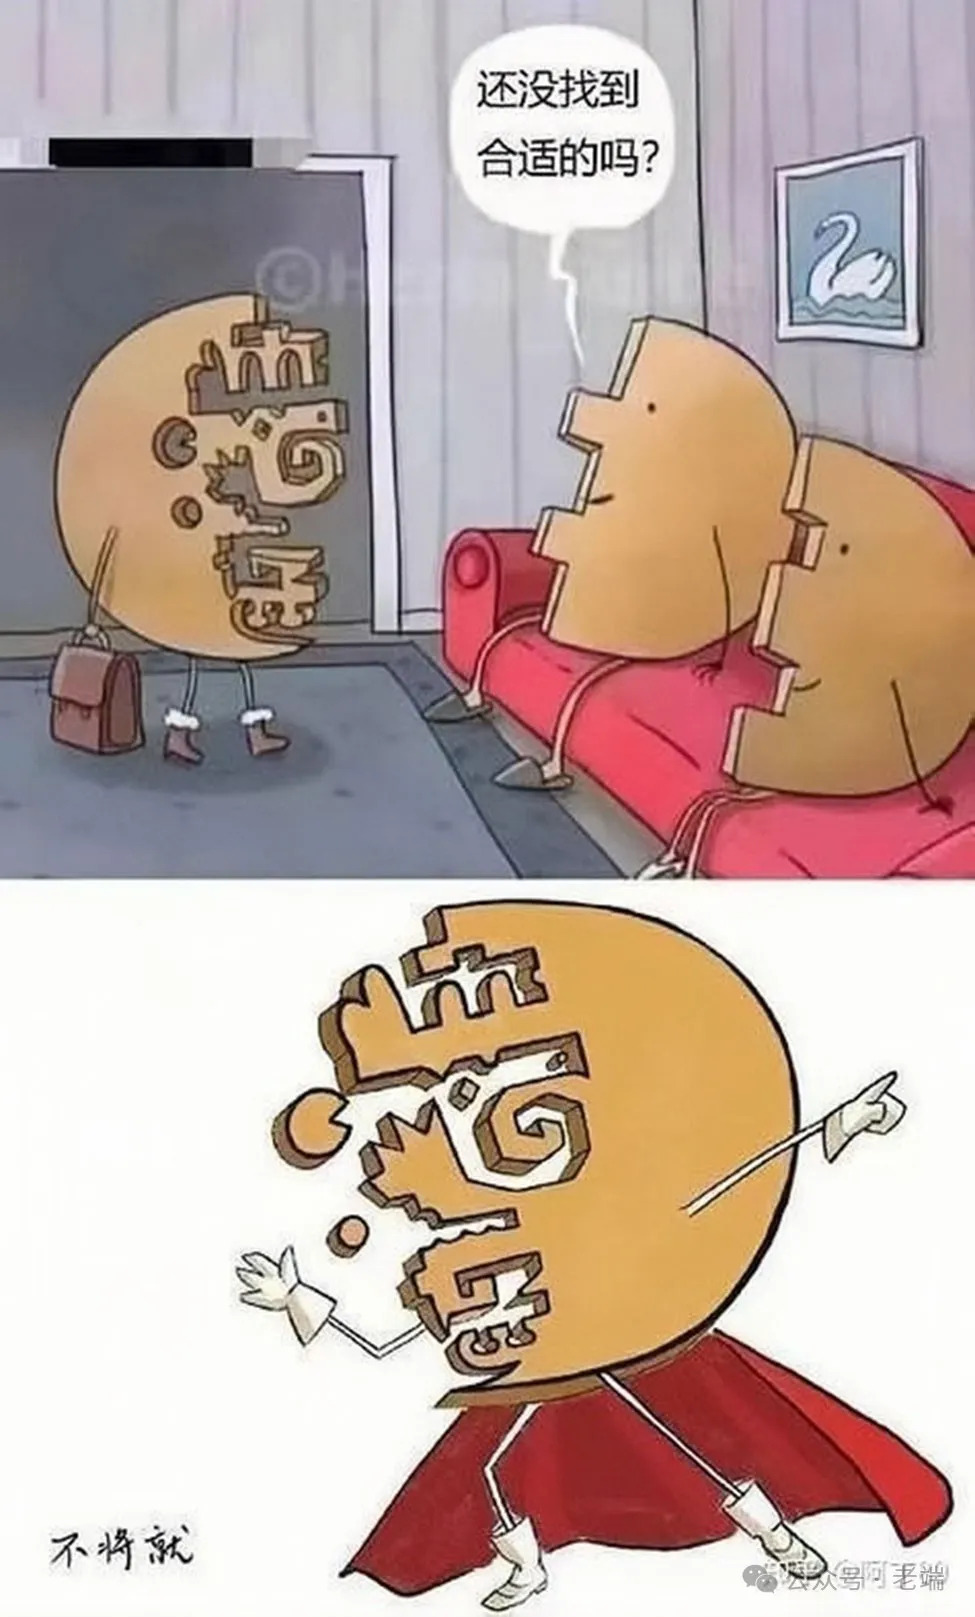
\includegraphics[width=7.5cm]{2024-04-24-001}
\end{figure}

父母问她:还没找到合适的吗?你看她这个复杂样子,能找到另一半吗?没有另一半能够匹配她,除了搞电信诈骗的犯罪分子。

她们中的很多人,从小就是喝毒鸡汤长大的,最喜欢看的是咪蒙的文章和曲曲的视频,比如:

《只有把自己当公主,男人才会对待公主一样宠你》

《爱你的男人不会在意你的容貌》

《爱你的男人会把你当女儿宠》

《他不为你花钱就是不爱你》

《好看的女孩,都自带烧钱属性》

《中国男人配不上中国女人》

《会撒娇的女人最好命》

《一个男人跟你讲道理,那他就不爱你》

《婚姻里,女人最不需要的就是勤快》

《我妈把我养得这么贵,不是给你洗碗的》

《好女人就是要爆男人金币》

《男人就是行走的ATM,你要做的就是让他吐钱》

毒鸡汤喝多了,是会把脑子给烧坏的,假如我是女人,我听完也会爽得飞起,但理性告诉我这根本不现实啊。这类毒鸡汤的核心就只有两条:

1,男人需要为婚姻提供所有物质基础,而我只需要拎包入住;

2,只要我什么都不付出,我就不会有损失。

这两条形成了一个逻辑闭环,那就是自己是没有任何问题的,可是如何解释还没能嫁出去呢?当然是国男太差,配不上自己。错的也不是我,而是这个世界。

女人找老公总是尽量向上看,但随着女人社会地位的提高,她们越来越多地参与男性的竞争并获得成功,这就使得大部分女人看得上的优秀男人特别稀少。一个年薪10万人民币的男人,在一线城市女性看来,是个十足的穷鬼,因为这个收入根本别想买房,起码要年薪20万起步。

但你知道吗,只要你年收入超过8万人民币,你在中国就可以排到顶层的5\%了。在全球范围来说,如果你年收入超过10万人民币,你可以排到顶层的2\%,换句话说已经超过了98\%的地球人。

让我说得再直白一些,剩女嫁不出去,最主要的原因是无法正确评估自己,又过高估计了适合匹配的男人。这些女性完全不会考虑阶层比自己低的男性,同一阶层的男人也看不上,比自己阶层高的男人数量又太少了,根本不够分,这才是大城市剩女遍地走的根本原因。

在这种情况下,男人也逐渐认清了现实,前段时间杭州举办了一场相亲大会,竟然没有一个男人报名参加,网友评论说:这是沸羊羊掀桌子了?其实不是沸羊羊掀桌子,而是男人醒悟了,与其跑去相亲大会被羞辱,还不如在家玩游戏。

从历史上看,光棍从来就只有男人,不可能有女人,因为在古代,你完全可以给地主做小妾,现在我们实行一夫一妻制了,小妾是做不成了,于是才会有女光棍。这也揭示了一个基本事实:我们所有人的祖先都是富人,因为穷人根本没有后代,不管你信不信,你的祖上都是大户。

这些人还特别听不得别人劝生,就像是身上的逆鳞,一碰就炸。但我说句实话,你结不结婚,生不生娃,除了你父母之外,其实没有人会关心。等到你父母也不在了,你就真的只剩下自己了。女性的预期寿命起码80岁吧,剩下这么长的日子你怎么过?

可能有些人会担心,如果大家都不婚不育,人口越来越少怎么办?我觉得你大可不必担心,因为真相是:大多数人都绝嗣,也不会影响人口增长。我这么说是有根据的,有一篇非常有趣的论文叫《延续香火的理想与普遍绝嗣的现实》,讲的就是这件事。

在明清时期,很多大家族喜欢修家谱,这些家谱很好地保留到了现在,论文研究的是《松源魏氏宗谱》,松源位于福建西北山区,相对比较闭塞,躲过了历次战乱。魏氏宗谱从明朝(1513年)开始修订,一直持续到民国(1917年),跨度长达四百年。

以下是研究发现:

在清朝长达三百年间,整个魏氏家族是逐步扩张的,从最初的169个男性发展到最后是1360个男性。不过每一代都有大量男性被淘汰出局(绝嗣),所以虽然总人数增长了8倍,但86.39\%的人都绝后了,换言之,最后这1360个后代,是由最初13.61\%的人留下的。

在这里我们得到一个重要结论,就算总人口增加了8倍,能留下后代的比例也就只有13.6\%,进一步研究发现,就算你站在了13.6\%的赢家队伍中,赢的程度也是不一样的,75\%的人最终留下的支脉数只有不到5个,但有三个成功者,他们分别留下了超过100个支脉。这属于是严重的贫富差距了。

看到这里,你当然很想知道那些成功者到底是怎么成功的。下面我们分析这些指标:生育子女数、妻子数、社会经济地位、夭折儿童数。

生育子女数是影响传嗣成功率的最主要因素,这个很容易理解,比较奇怪的是老婆数量对传嗣成功率竟然影响不大。一般认为老婆越多,子女也越多,但竟然得不到统计数据支持。

一个可能的原因是,古代女性十几岁就可以嫁人生孩子,一个女人足够生下十个孩子,但其中多数都不可能活到成年,所以瓶颈不在女人的生育力,而在于能否养大成人。

社会经济地位是影响传嗣成功率的最主要因素,因为穷人在婚姻市场上处于劣势地位,女性十几岁就可以嫁人,但古代男性活到三四十岁才娶妻是很平常的,一辈子打光棍也不少见。有钱人家的儿子,20岁就可以娶妻生子,穷人混到40岁才娶老婆,那差别就大了。前者有几十年的生育期,后者的生育期就只剩下几年了。

社会经济地位高的家庭,孩子也不容易出现营养不良,营养不良是导致夭折的主要因素,营养不良的孩子更容易感染各种传染病。穷人生了孩子,如果感觉养不活,要么送人,要么卖掉,甚至还会杀婴。

家谱中并不会记录此人一年赚多少钱,那么我们怎么判断他的社会经济地位呢?方法是用“族长”判断经济地位,用“功名”判断社会地位。族长拥有家族中资源的分配权,必定是掌握资源最多的那一支的代表。功名就是念书的成就,有没有考中秀才、举人和进士。因为只有家里有钱,才能供孩子全脱产念书,穷人是念不起书的,所以考取了功名必然意味着家庭经济条件不错。同时,考取了功名就意味着有可能做官,社会地位大大增加了。

中国传统是不孝有三无后为大,但事实上多数人都是无后的,只有少数人(13.61\%)能在300年后还留有后代。这就意味着,传宗接代是理想,绝嗣才是现实。

正因为只有少数男人才能留下后代,所以女人也进化出了相关的适应性,那就是针对高社会经济地位男人的偏好。因为人都是慕强的,和这些男人结婚,才能最大化自身的繁衍成就。如果不能嫁给这些人,而是嫁给穷屌丝,那跟绝后也没什么区别。

现代社会如此规模的女性终身不婚,这在历史上是极为罕见的,不想嫁给屌丝,这没问题,但有钱人数量就这么多,现在也不能纳妾,做小三风险又大,那还能怎么办呢?我的看法是无解。

最后我想说,我不会劝任何人生孩子,反而鼓励大家不婚不育,因为这样一来,你们空出来的资源才能给那些生孩子的人,他们的娃将来才不会内卷。所以,在生不生这个问题上,我们达成了一致——不生!

不过我自己还打算继续生下去,我群里的读者大部分都是二胎起步,三胎、四胎也不少见,他们觉得我说的对就行了。而且我再告诉你一个冷知识,生一胎是最累的,生多了反而不累,因为只生一个,你就输不起了,心态上必须紧绷,你就只能鸡娃,那能不累么?生多了,心态好得多,根本不鸡娃,娃和你都开心。

\end{document}

